\subsubsection{UAP ResNet18} \label{chap:UAP ResNet18}
In diesem Kapitel werden die durch das ResNet18 Modell erstellten \acrshort{uap} visualisiert. Das Modell wurde mit den Datensätzen \nameref{chap:COVIDx CXR-4} und \nameref{chap:Hirntumor} trainiert.

Die Anzahl der pro Modell generierten \acrshort{uap} hängt vom Parameter $i$ (Anzahl der zu generierenden Perturbationsbilder) ab. Daher existieren pro Robustifikationslevel fünf \acrshort{uap}. In den Abbildungen \ref{fig:uap-vor-nach-resnet18}, \ref{fig:uap-verlauf-resnet18-covid-robustifikation} und \ref{fig:uap-verlauf-resnet18-mri-robustifikation}, wird jeweils die erste \acrshort{uap} mit dem Index 0 dargestellt. Die weiteren Indizes sind im Anhang dargestellt und können unter den Abbildungen \ref{fig-appendix:uap-resnet18-covid-rest} und \ref{fig-appendix:uap-resnet18-hirntumor-rest} eingesehen werden.

\todo{Anhang mit Bilder erstellen}

% UAP ResNet18 Covidx CXR-4
\begin{figure}[H]
    \centering
        \begin{subfigure}{0.19\linewidth}
            \centering
            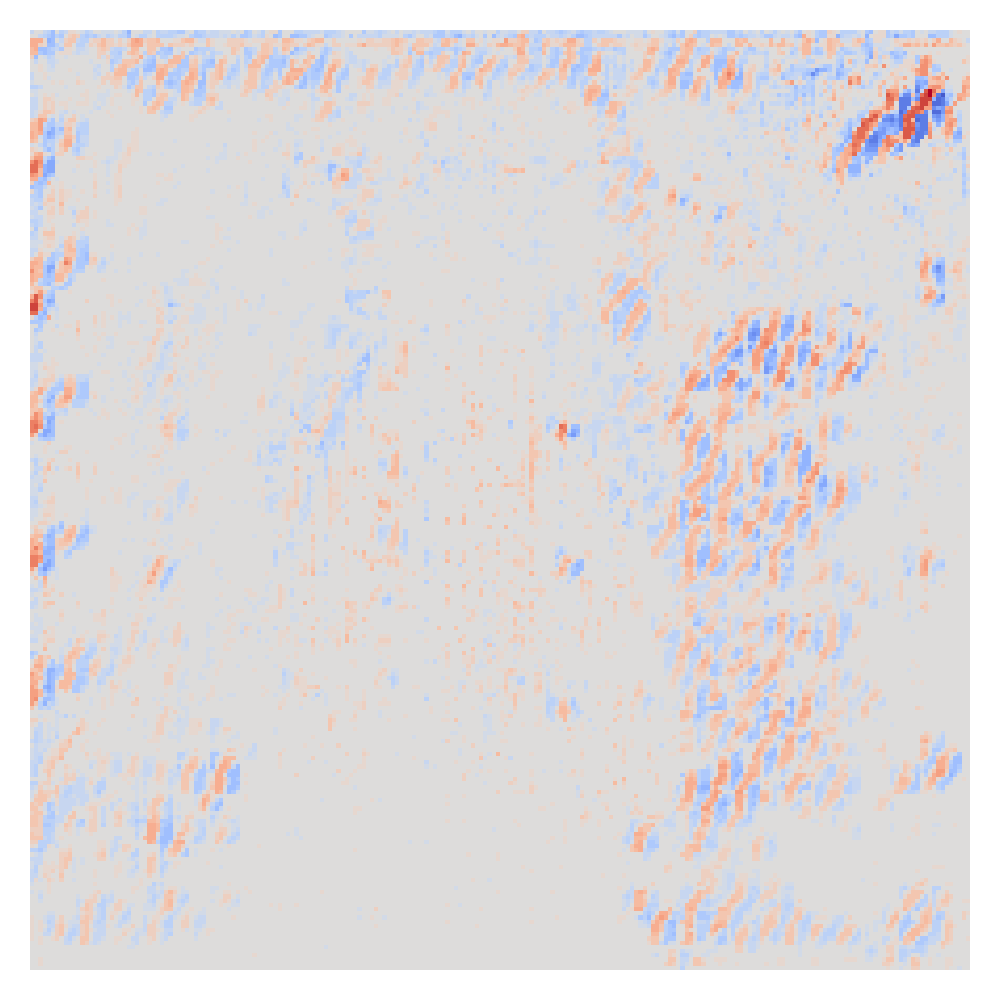
\includegraphics[height=1\linewidth]{01-images/05-resultate/uap_resnet18/uap0-resnet18-covidx_data-n200-robustificationslevel0.png}
        \end{subfigure}\hfill%
        \begin{subfigure}{0.19\linewidth}
            \centering
            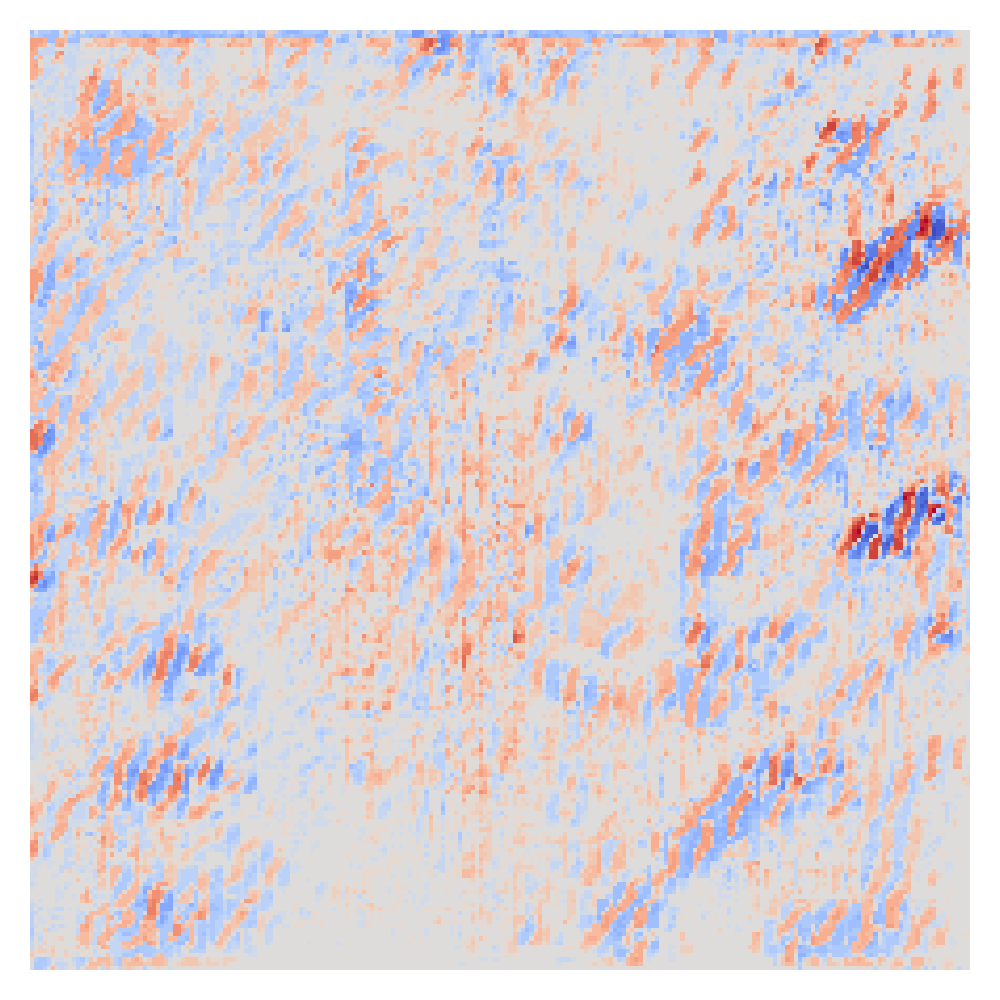
\includegraphics[height=1\linewidth]{01-images/05-resultate/uap_resnet18/uap1-resnet18-covidx_data-n200-robustificationslevel0.png}
        \end{subfigure}\hfill%
        \begin{subfigure}{0.19\linewidth}
            \centering
            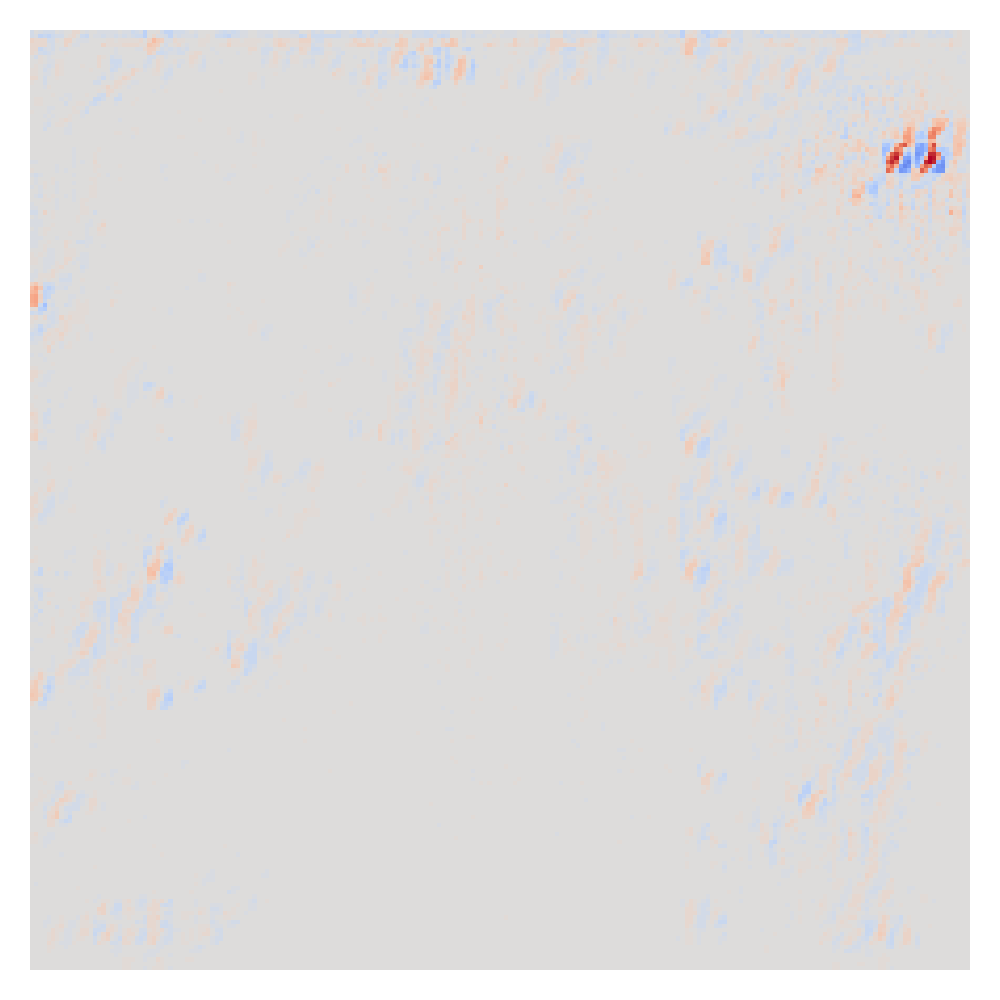
\includegraphics[height=1\linewidth]{01-images/05-resultate/uap_resnet18/uap2-resnet18-covidx_data-n200-robustificationslevel0.png}
        \end{subfigure}\hfill%
        \begin{subfigure}{0.19\linewidth}
            \centering
            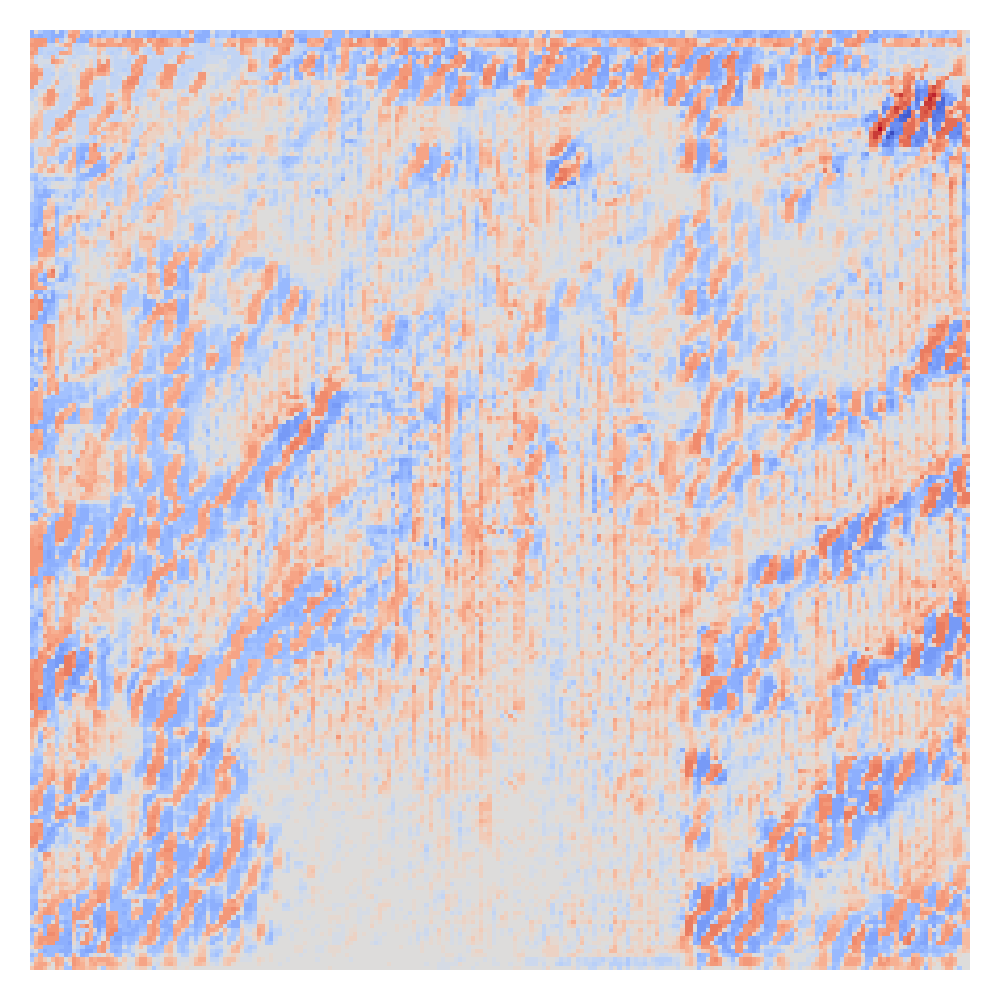
\includegraphics[height=1\linewidth]{01-images/05-resultate/uap_resnet18/uap3-resnet18-covidx_data-n200-robustificationslevel0.png}
        \end{subfigure}\hfill%
        \begin{subfigure}{0.19\linewidth}
            \centering
            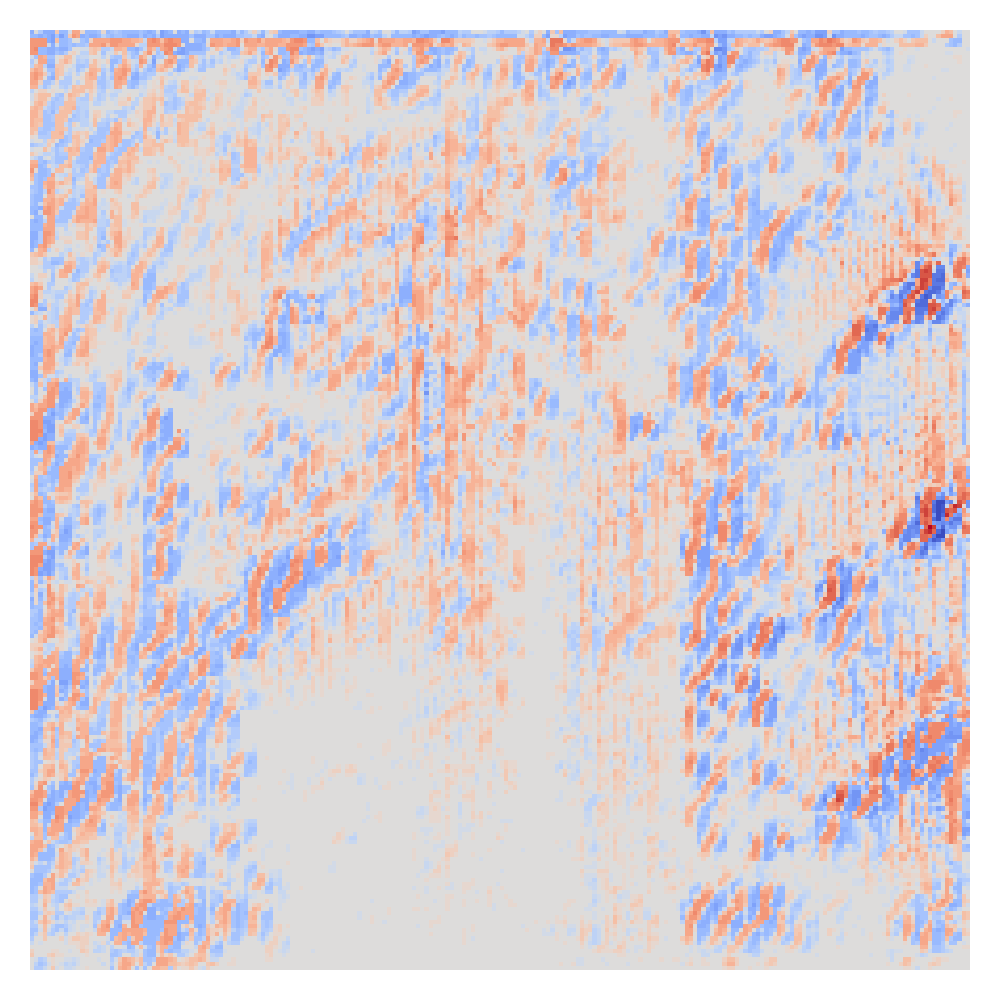
\includegraphics[height=1\linewidth]{01-images/05-resultate/uap_resnet18/uap4-resnet18-covidx_data-n200-robustificationslevel0.png}
        \end{subfigure}
    \caption{Fünf unterschiedliche UAP, generierte durch gemischte Teilmenge aller positiven gelabelten Trainingsbilder $X_{\text{train},+,1:n}$ von ResNet18, trainiert auf COVIDx CXR-4 Datensatz.}
    \label{fig:uap-resnet18-covidx-robustification-0}
\end{figure}

% UAP ResNet18 MRI
\begin{figure}[H]
    \centering
        \begin{subfigure}{0.19\linewidth}
            \centering
            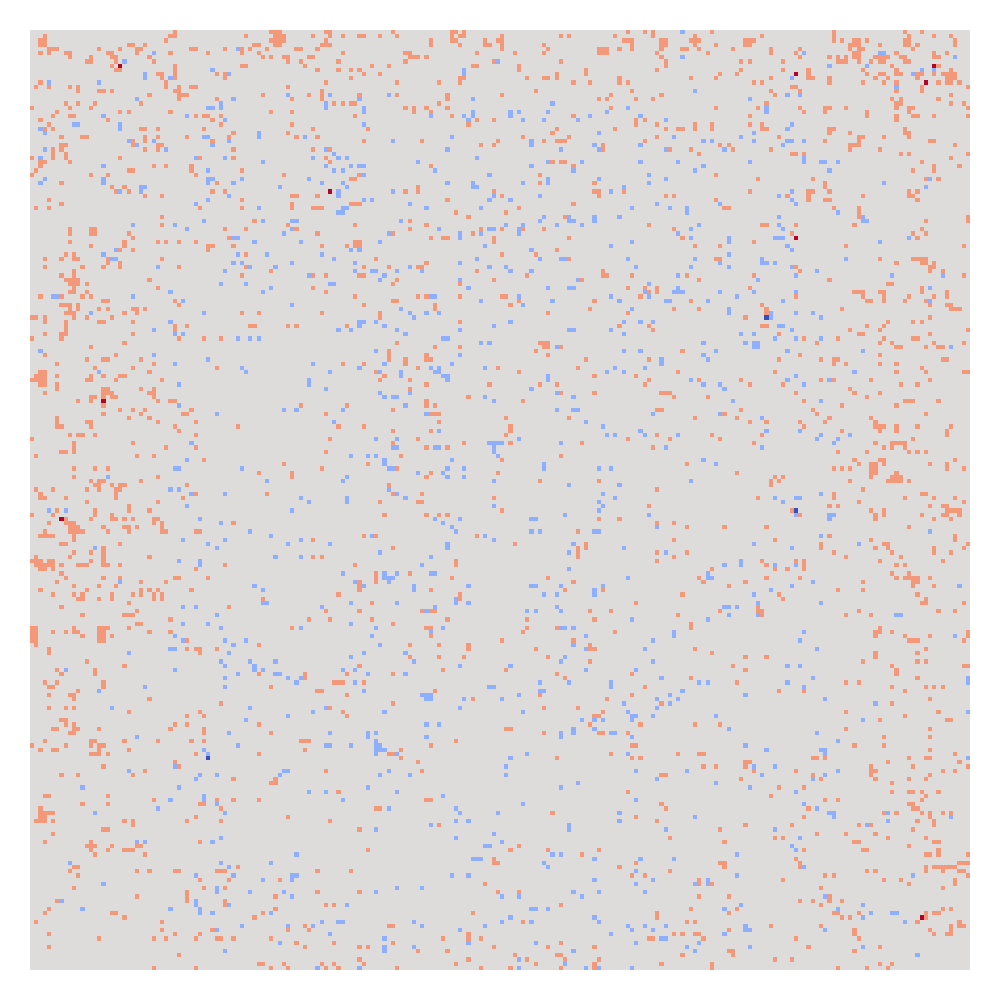
\includegraphics[height=1\linewidth]{01-images/05-resultate/uap_resnet18/uap0-resnet18-mri_data-n200-robustificationslevel0.png}
        \end{subfigure}\hfill%
        \begin{subfigure}{0.19\linewidth}
            \centering
            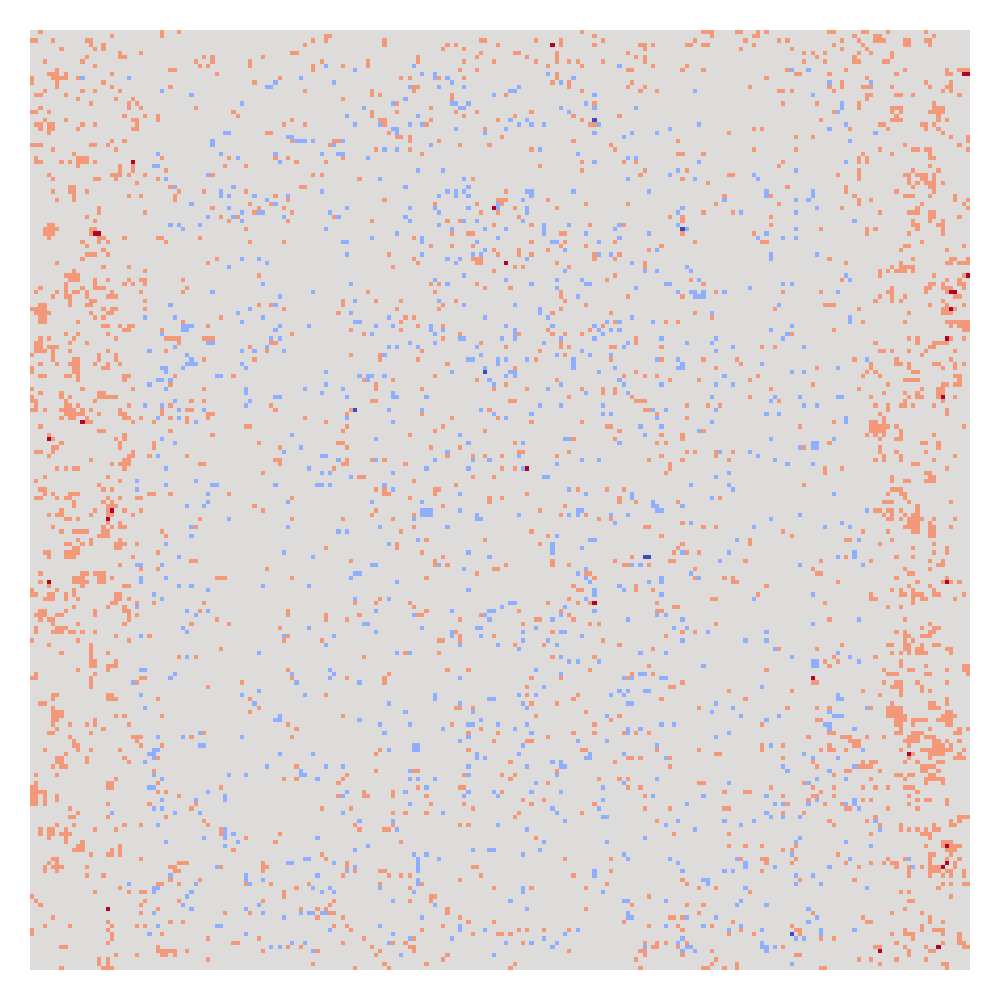
\includegraphics[height=1\linewidth]{01-images/05-resultate/uap_resnet18/uap1-resnet18-mri_data-n200-robustificationslevel0.png}
        \end{subfigure}\hfill%
        \begin{subfigure}{0.19\linewidth}
            \centering
            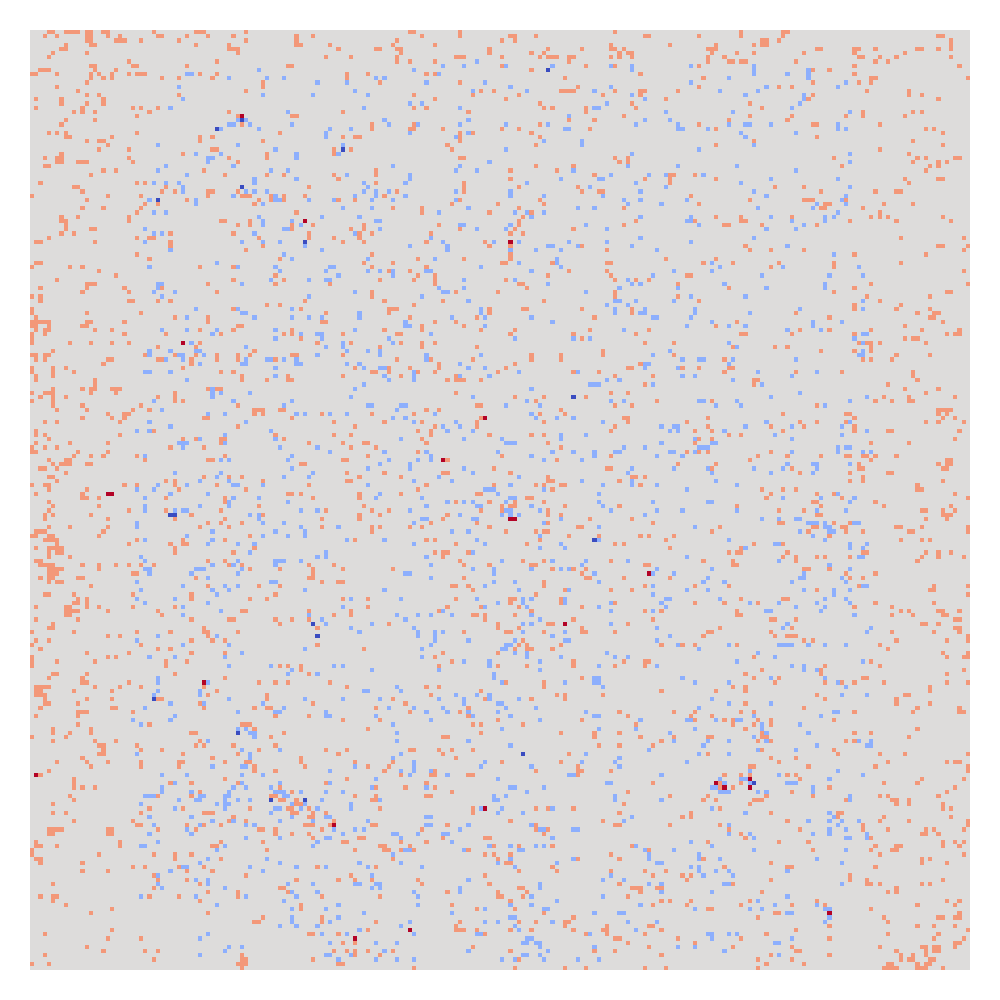
\includegraphics[height=1\linewidth]{01-images/05-resultate/uap_resnet18/uap2-resnet18-mri_data-n200-robustificationslevel0.png}
        \end{subfigure}\hfill%
        \begin{subfigure}{0.19\linewidth}
            \centering
            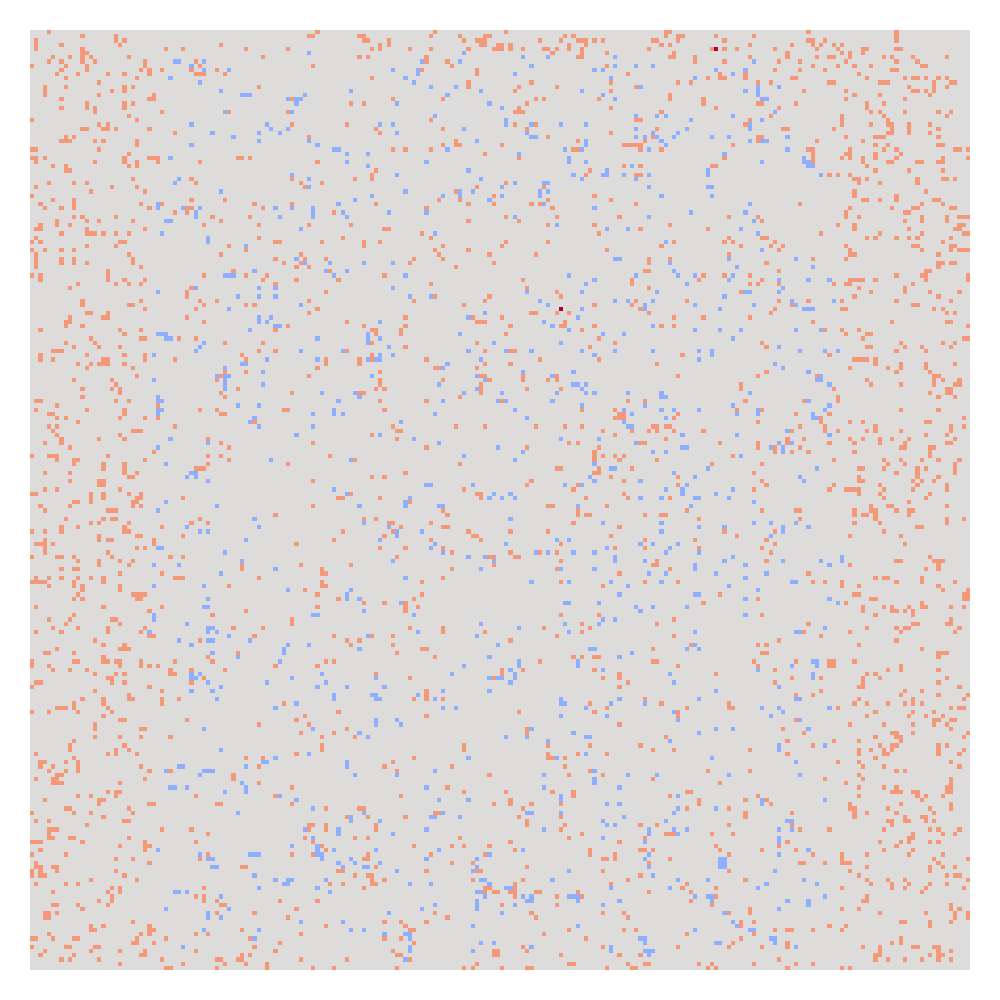
\includegraphics[height=1\linewidth]{01-images/05-resultate/uap_resnet18/uap3-resnet18-mri_data-n200-robustificationslevel0.png}
        \end{subfigure}\hfill%
        \begin{subfigure}{0.19\linewidth}
            \centering
            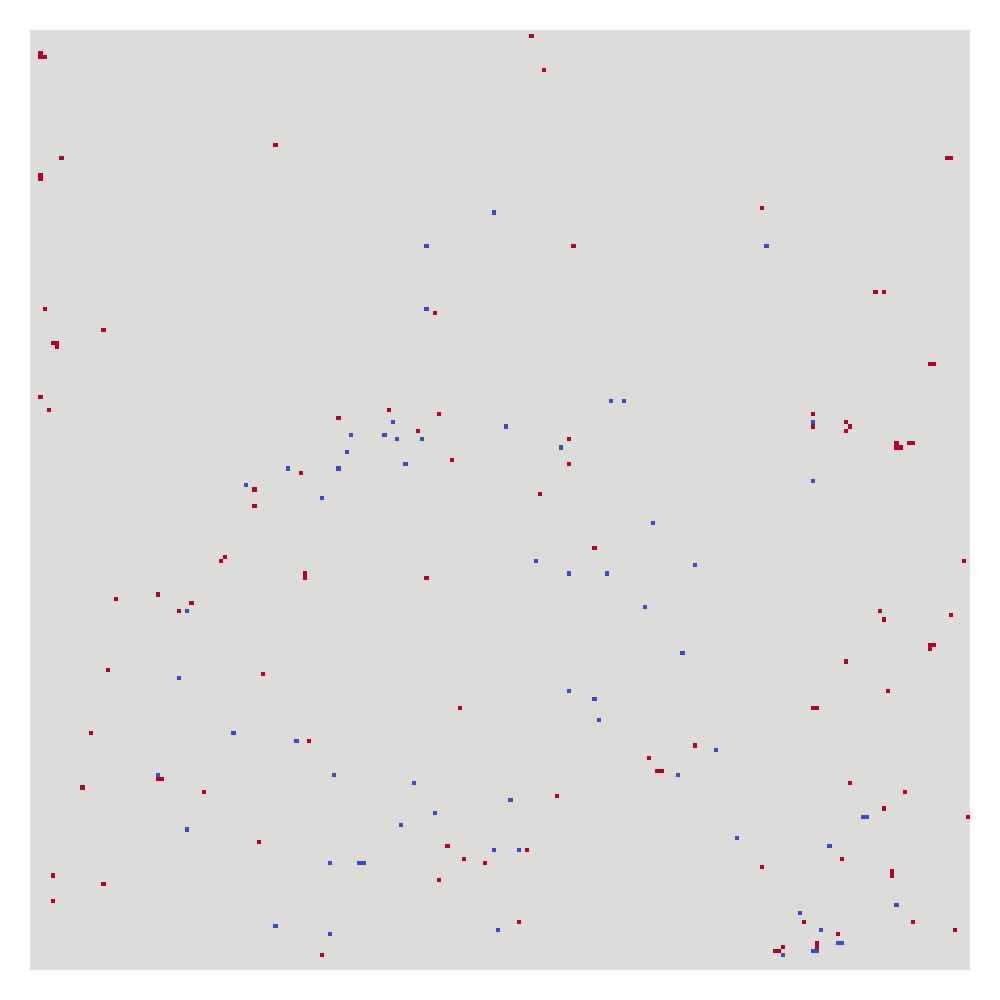
\includegraphics[height=1\linewidth]{01-images/05-resultate/uap_resnet18/uap4-resnet18-mri_data-n200-robustificationslevel0.png}
        \end{subfigure}
    \caption{Fünf unterschiedliche UAP, generierte durch gemischte Teilmenge aller positiven gelabelten Trainingsbilder $X_{\text{train},+,1:n}$ von ResNet18, trainiert auf Hirntumor Datensatz.}
    \label{fig:uap-resnet18-mri-robustification-0}
\end{figure}

% UAP vor und nach Robustifikation
\begin{figure}[H]
    \centering
    \captionsetup{justification=centering}
    \begin{subfigure}{0.19\linewidth}
        \centering
        \text{Vor}\\
        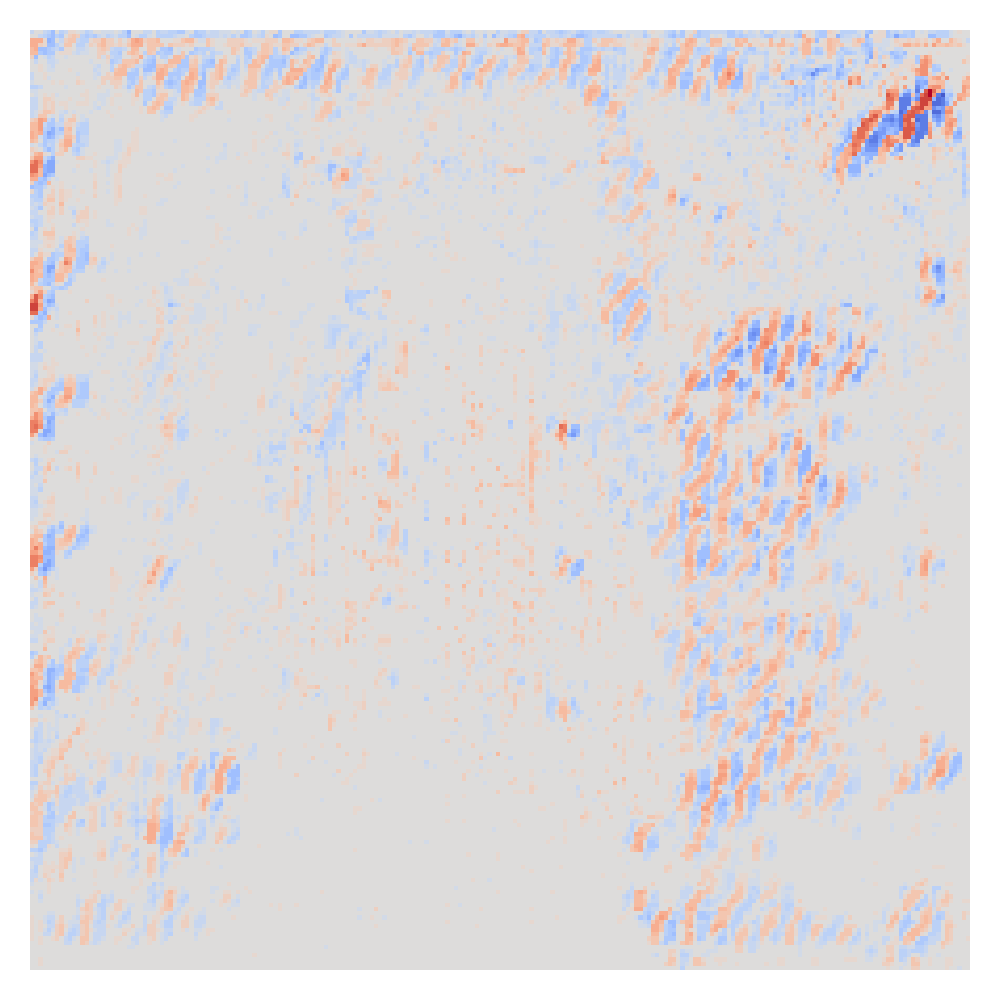
\includegraphics[width=\linewidth]{01-images/05-resultate/uap_resnet18/uap0-resnet18-covidx_data-n200-robustificationslevel0.png}
        \caption{ResNet18 \\Covidx CXR-4}
    \end{subfigure}
    \hfill%
    \begin{subfigure}{0.19\linewidth}
        \centering
        \text{Nach}\\
        
\includegraphics[width=\linewidth]{01-images/05-resultate/uap_resnet18/uap0-resnet18-covidx_data-n200-robustificationslevel9.png}
        \caption{ResNet18 \\Covidx CXR-4}
    \end{subfigure}
    \hfill%
    \begin{subfigure}{0.19\linewidth}
        \centering
        \text{Vor} \\
        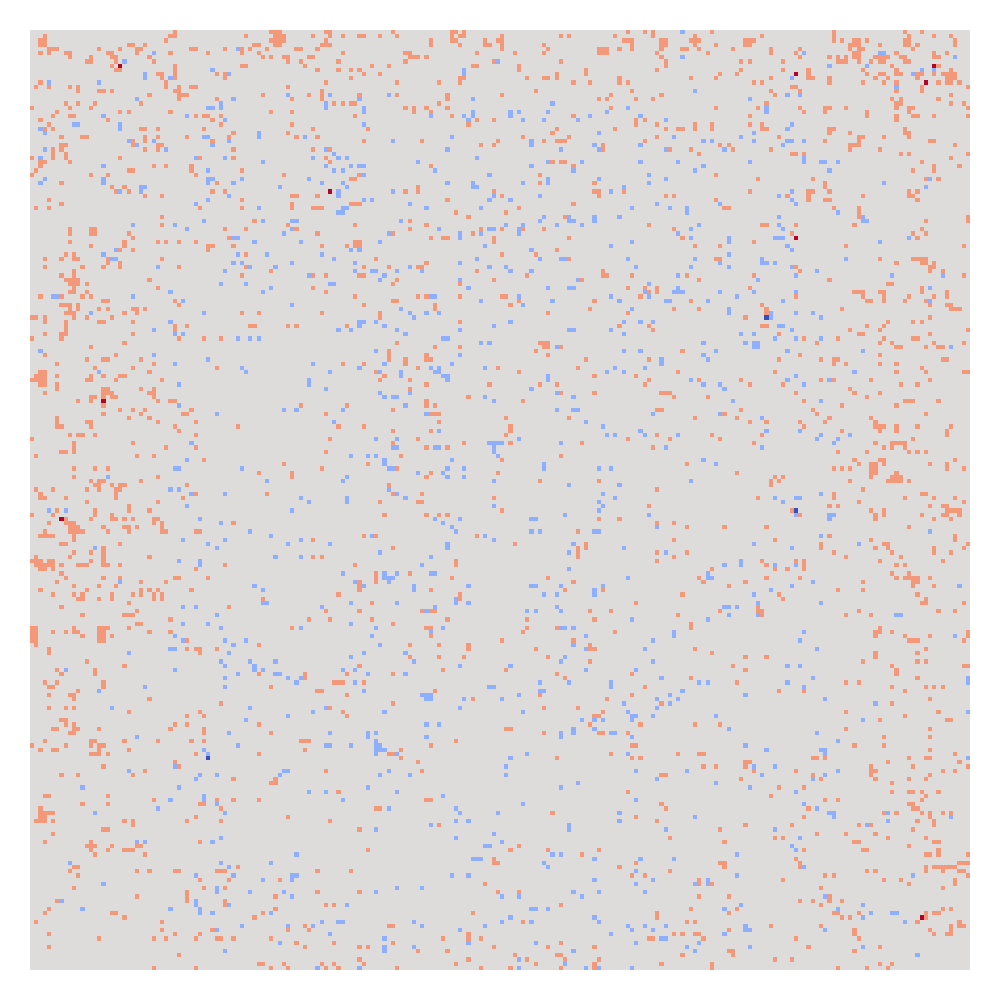
\includegraphics[width=\linewidth]{01-images/05-resultate/uap_resnet18/uap0-resnet18-mri_data-n200-robustificationslevel0.png}
        \caption{ResNet18 \\ Hirntumor}
    \end{subfigure}
    \hfill%
    \begin{subfigure}{0.19\linewidth}
        \centering
        \text{Nach}\\
        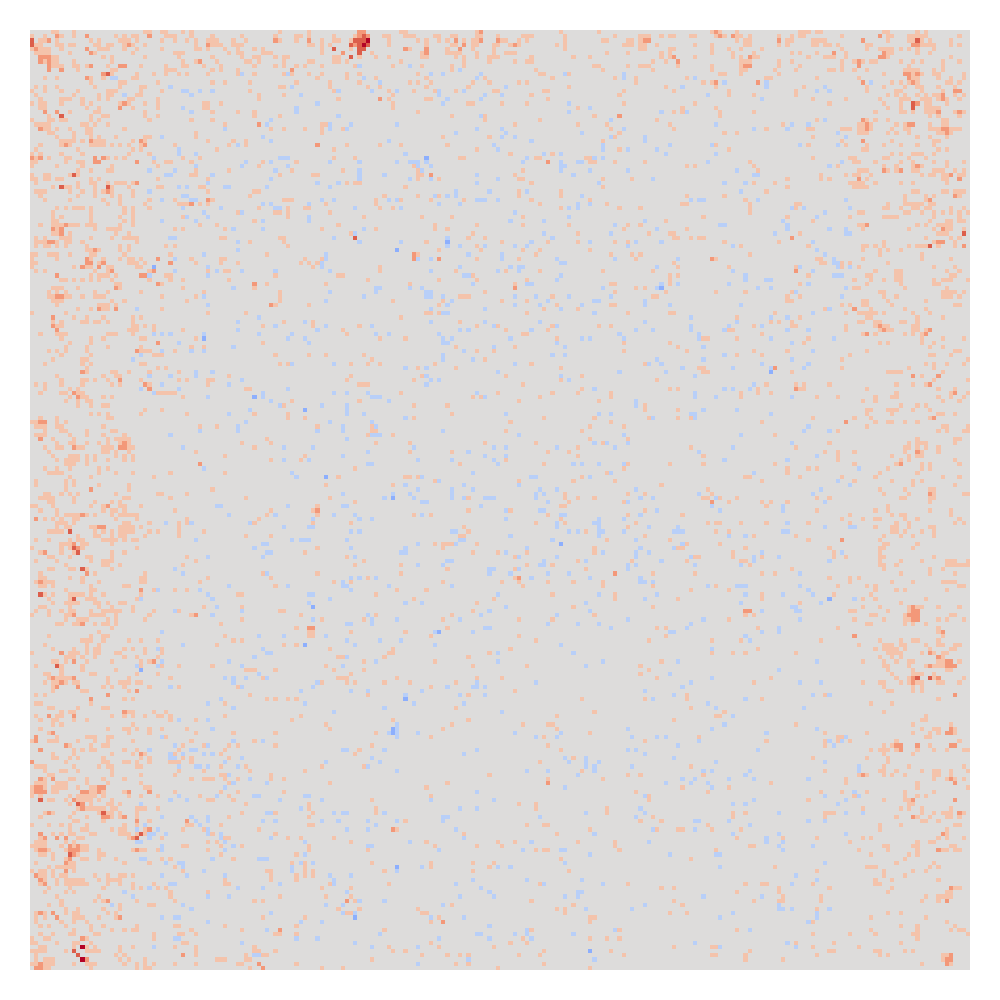
\includegraphics[width=\linewidth]{01-images/05-resultate/uap_resnet18/uap0-resnet18-mri_data-n200-robustificationslevel6.png}
        \caption{ResNet18 \\ Hirntumor}
    \end{subfigure}
    \caption{UAP vor und nach Modell Robustifikation durch Adversarial Training}
    \label{fig:uap-vor-nach-resnet18}
\end{figure}

% UAP Robustifikationslevel Covidx CXR-4
\begin{figure}[H]
    \centering
    \text{Entwicklung der UAP durch Adversarial Attack und Adversarial Training} \\
    \begin{subfigure}{0.095\linewidth}
        \centering
        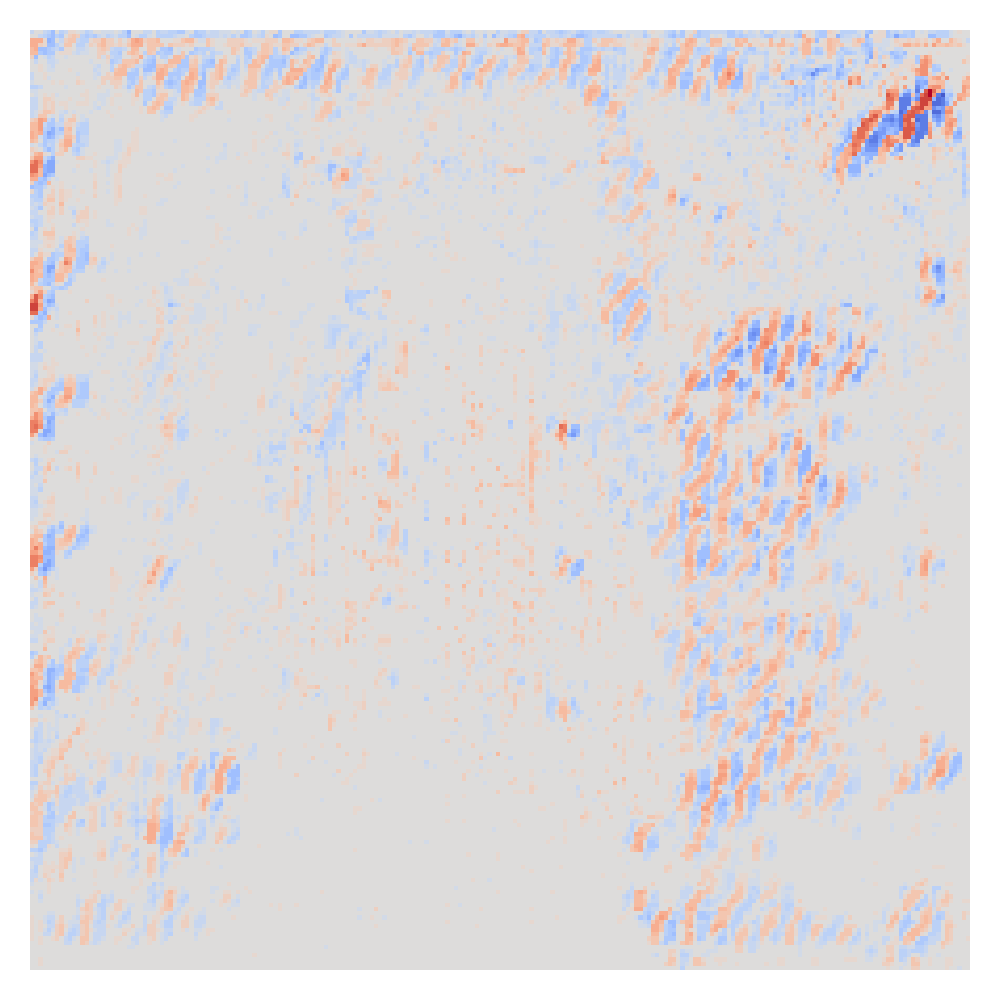
\includegraphics[height=1\linewidth]{01-images/05-resultate/uap_resnet18/uap0-resnet18-covidx_data-n200-robustificationslevel0.png}
    \end{subfigure}\hfill%
    \begin{subfigure}{0.095\linewidth}
        \centering
        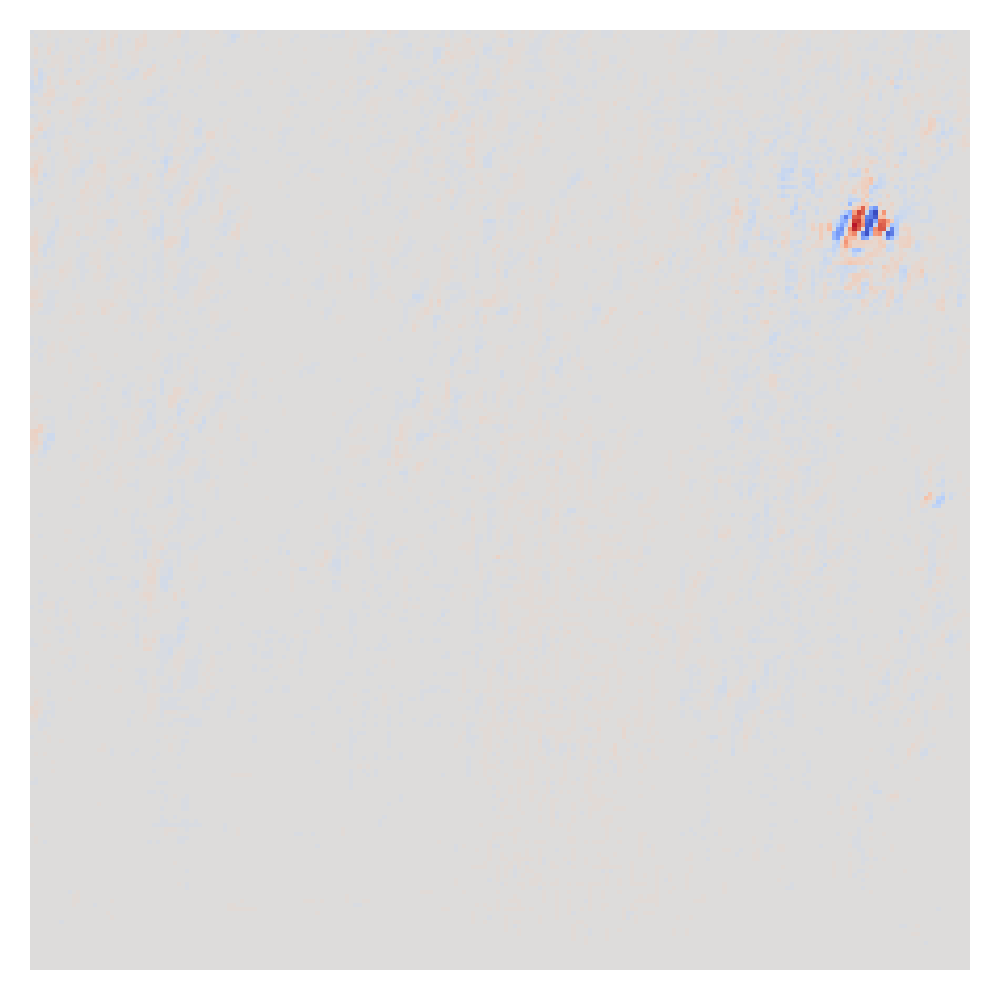
\includegraphics[height=1\linewidth]{01-images/05-resultate/uap_resnet18/uap0-resnet18-covidx_data-n200-robustificationslevel1.png}
    \end{subfigure}\hfill%
    \begin{subfigure}{0.095\linewidth}
        \centering
        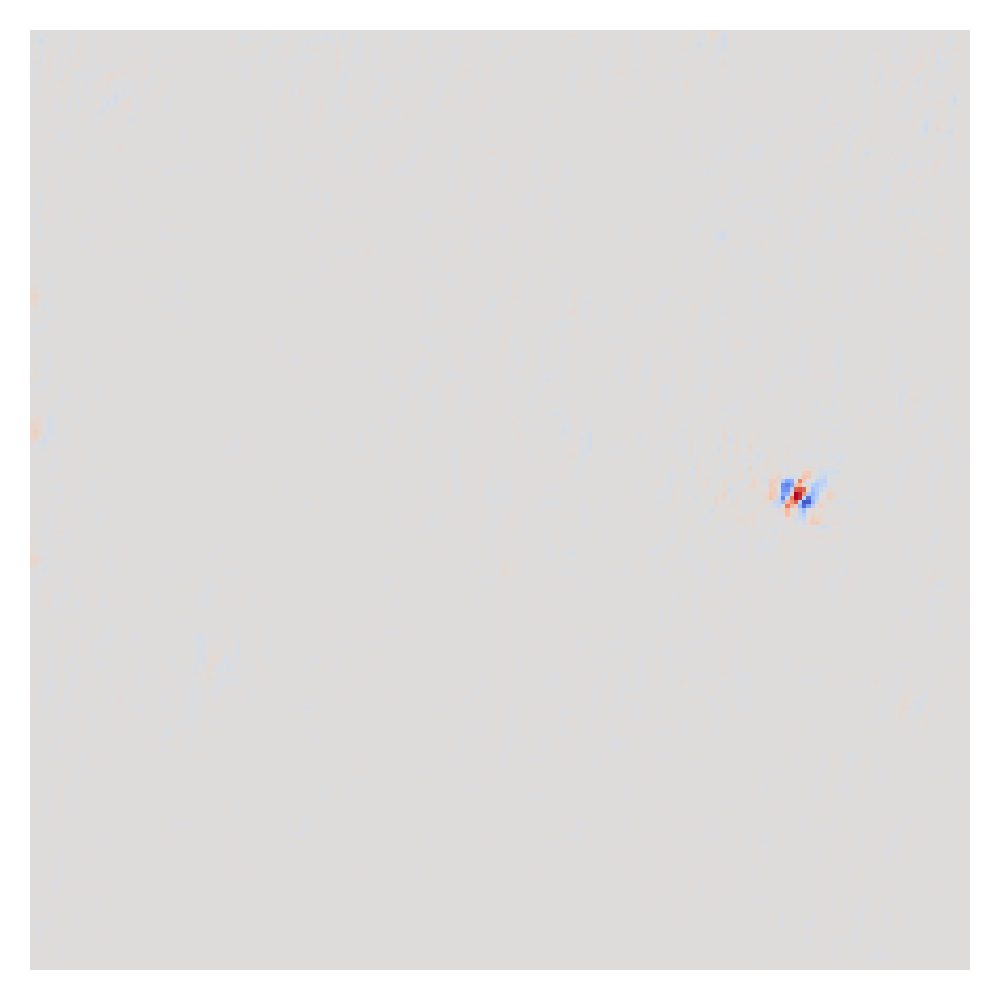
\includegraphics[height=1\linewidth]{01-images/05-resultate/uap_resnet18/uap0-resnet18-covidx_data-n200-robustificationslevel2.png}
    \end{subfigure}\hfill%
    \begin{subfigure}{0.095\linewidth}
        \centering
        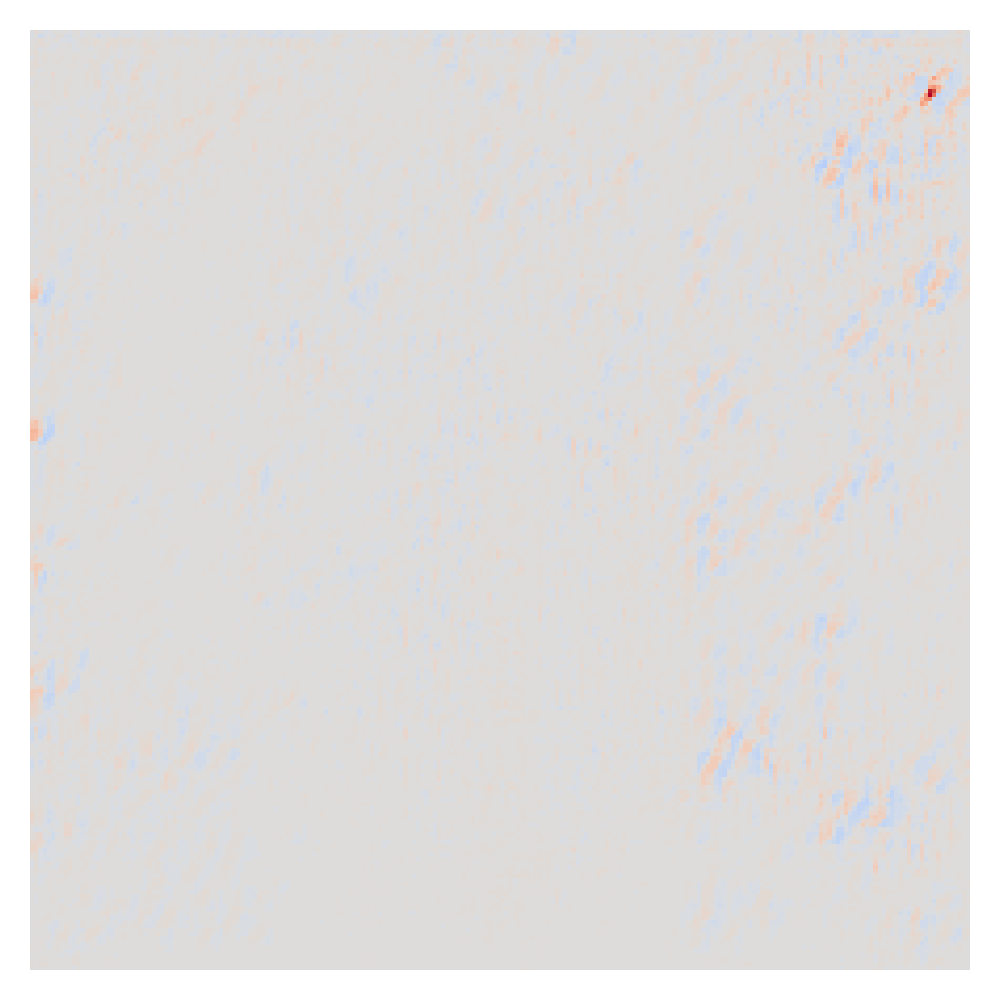
\includegraphics[height=1\linewidth]{01-images/05-resultate/uap_resnet18/uap0-resnet18-covidx_data-n200-robustificationslevel3.png}
    \end{subfigure}\hfill%
    \begin{subfigure}{0.095\linewidth}
        \centering
        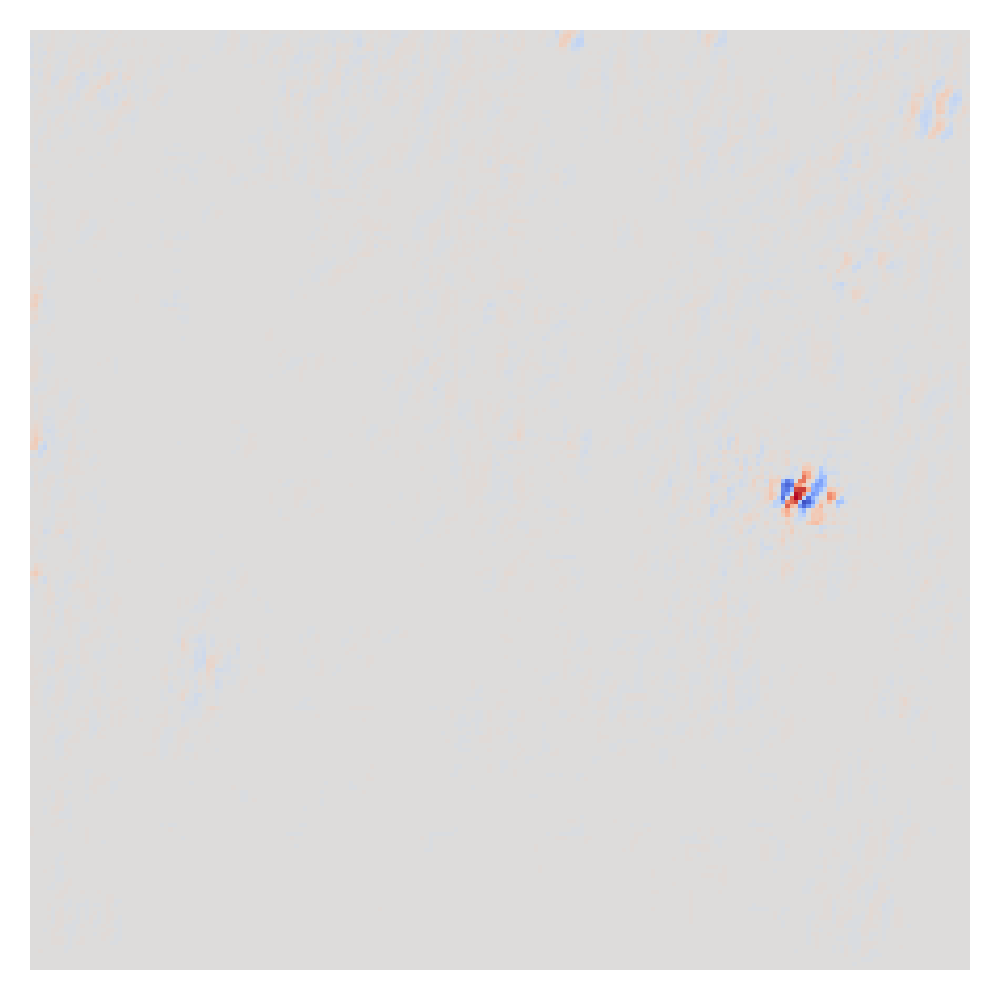
\includegraphics[height=1\linewidth]{01-images/05-resultate/uap_resnet18/uap0-resnet18-covidx_data-n200-robustificationslevel4.png}
    \end{subfigure}\hfill%
    \begin{subfigure}{0.095\linewidth}
        \centering
        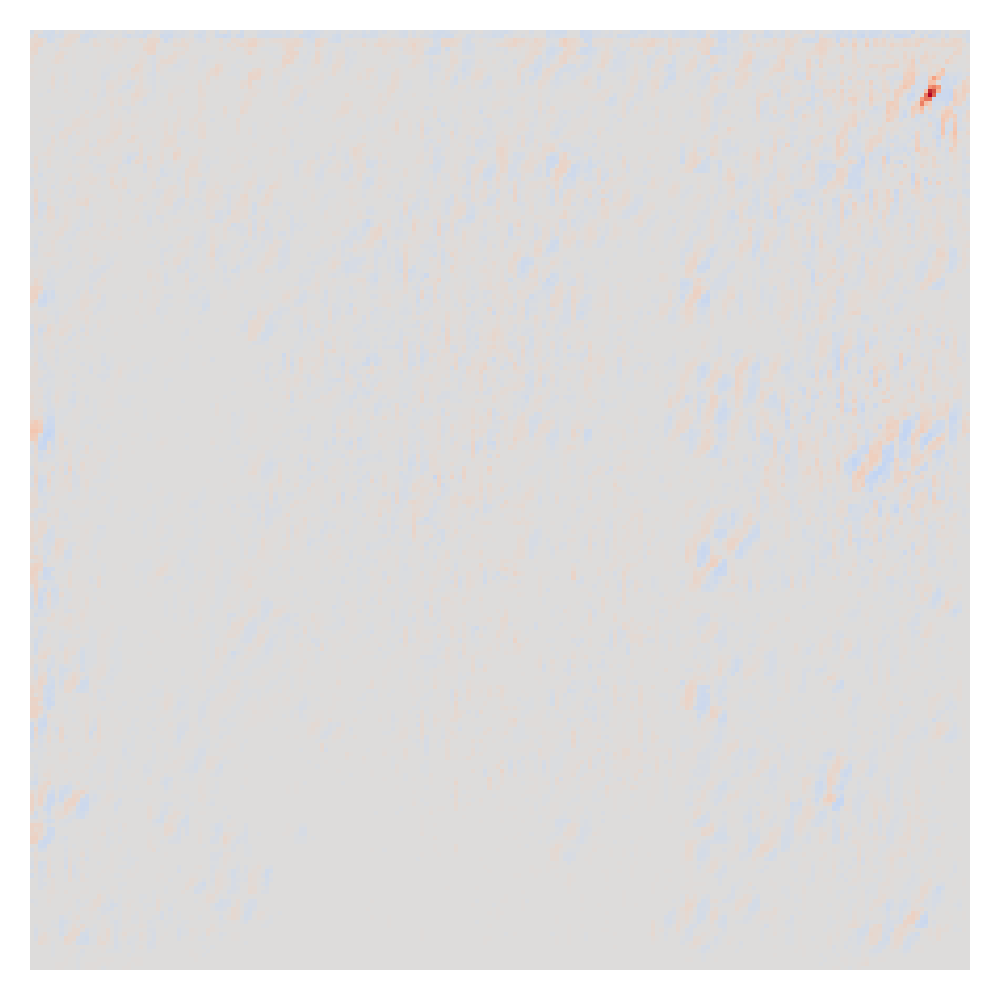
\includegraphics[height=1\linewidth]{01-images/05-resultate/uap_resnet18/uap0-resnet18-covidx_data-n200-robustificationslevel5.png}
    \end{subfigure}\hfill%
    \begin{subfigure}{0.095\linewidth}
        \centering
        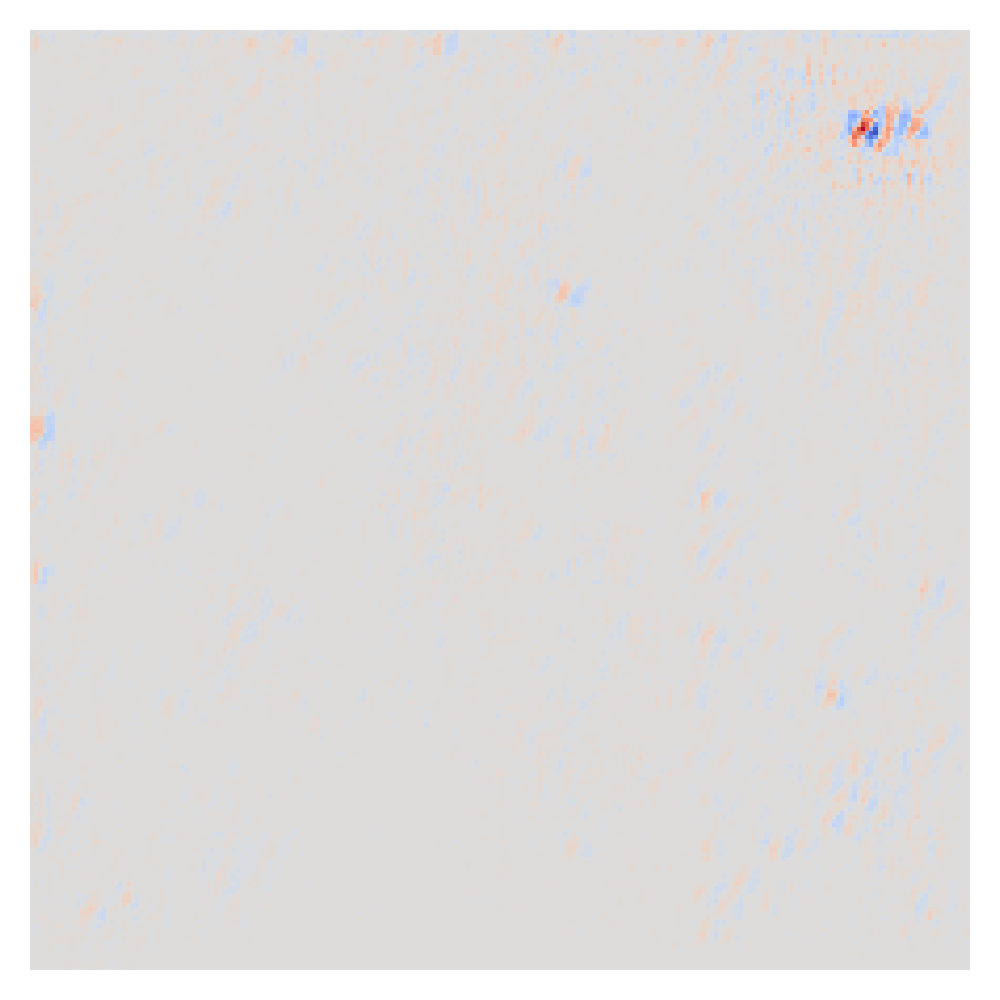
\includegraphics[height=1\linewidth]{01-images/05-resultate/uap_resnet18/uap0-resnet18-covidx_data-n200-robustificationslevel6.png}
    \end{subfigure}\hfill%
    \begin{subfigure}{0.095\linewidth}
        \centering
        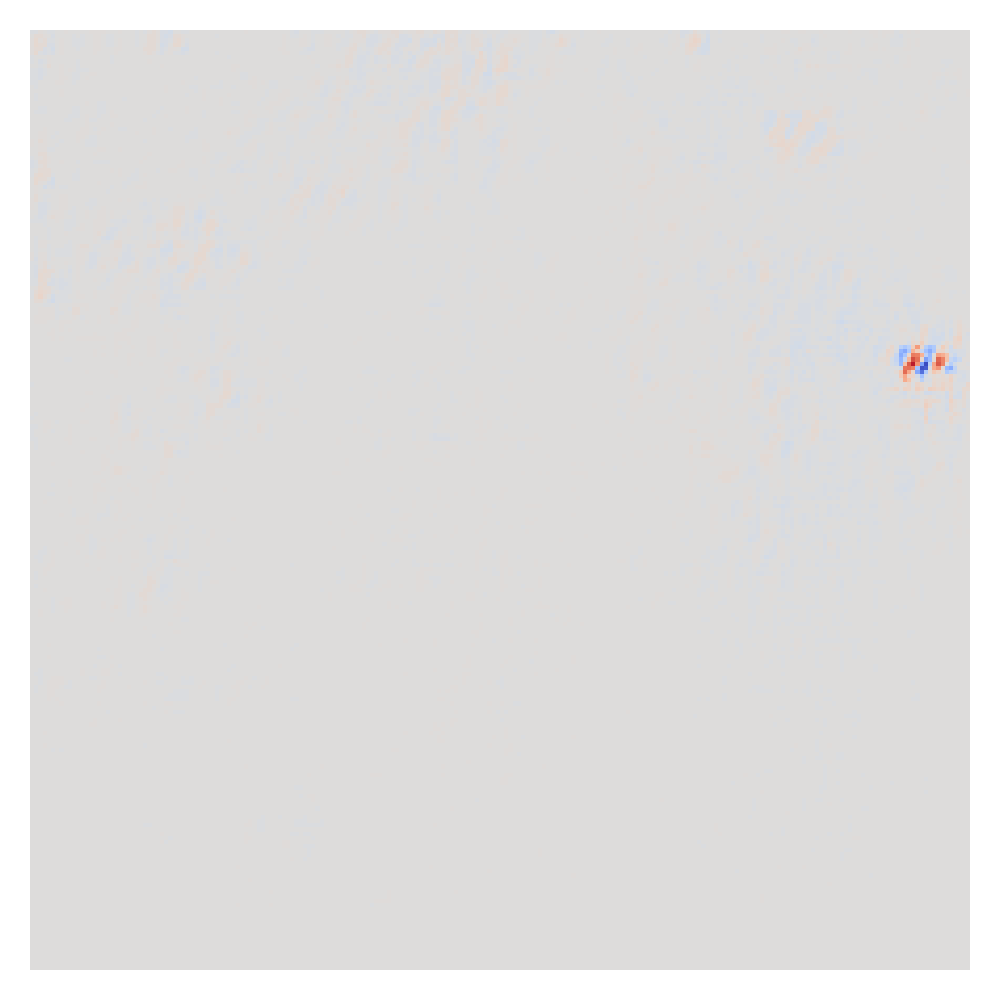
\includegraphics[height=1\linewidth]{01-images/05-resultate/uap_resnet18/uap0-resnet18-covidx_data-n200-robustificationslevel7.png}
    \end{subfigure}\hfill%
    \begin{subfigure}{0.095\linewidth}
        \centering
        
\includegraphics[height=1\linewidth]{01-images/05-resultate/uap_resnet18/uap0-resnet18-covidx_data-n200-robustificationslevel8.png}
    \end{subfigure}\hfill%
    \begin{subfigure}{0.095\linewidth}
        \centering
        
\includegraphics[height=1\linewidth]{01-images/05-resultate/uap_resnet18/uap0-resnet18-covidx_data-n200-robustificationslevel9.png}
    \end{subfigure}
    \caption{Generierte UAPs des mit ResNet18 trainierten Covidx CXR-4 Datensatzes nach jedem Robustifikationslevel durch Adversarial Training von links nach rechts.}
    \label{fig:uap-verlauf-resnet18-covid-robustifikation}
\end{figure}

% UAP Robustifikationslevel MRI
\begin{figure}[H]
    \centering
    \text{Entwicklung der UAP durch Adversarial Attack und Adversarial Training} \\
    \begin{subfigure}{0.095\linewidth}
        \centering
        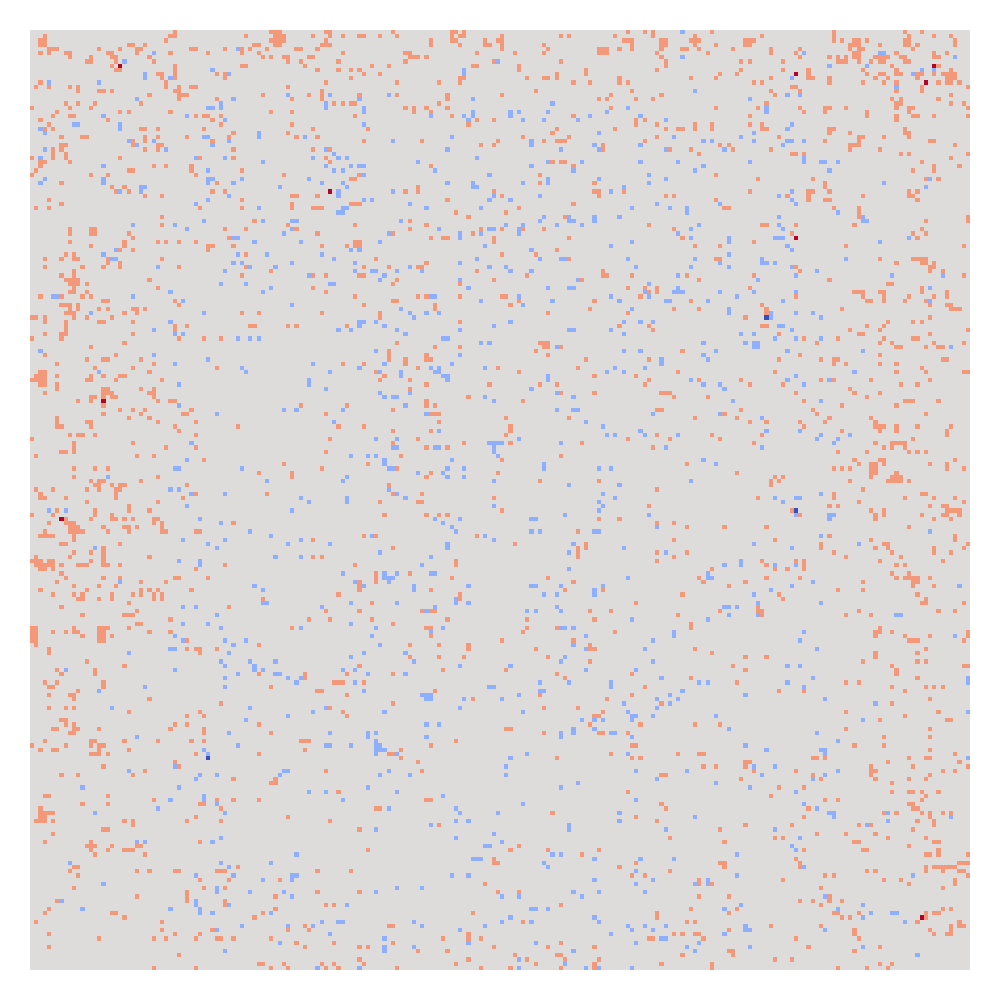
\includegraphics[height=1\linewidth]{01-images/05-resultate/uap_resnet18/uap0-resnet18-mri_data-n200-robustificationslevel0.png}
    \end{subfigure}\hfill%
    \begin{subfigure}{0.095\linewidth}
        \centering
        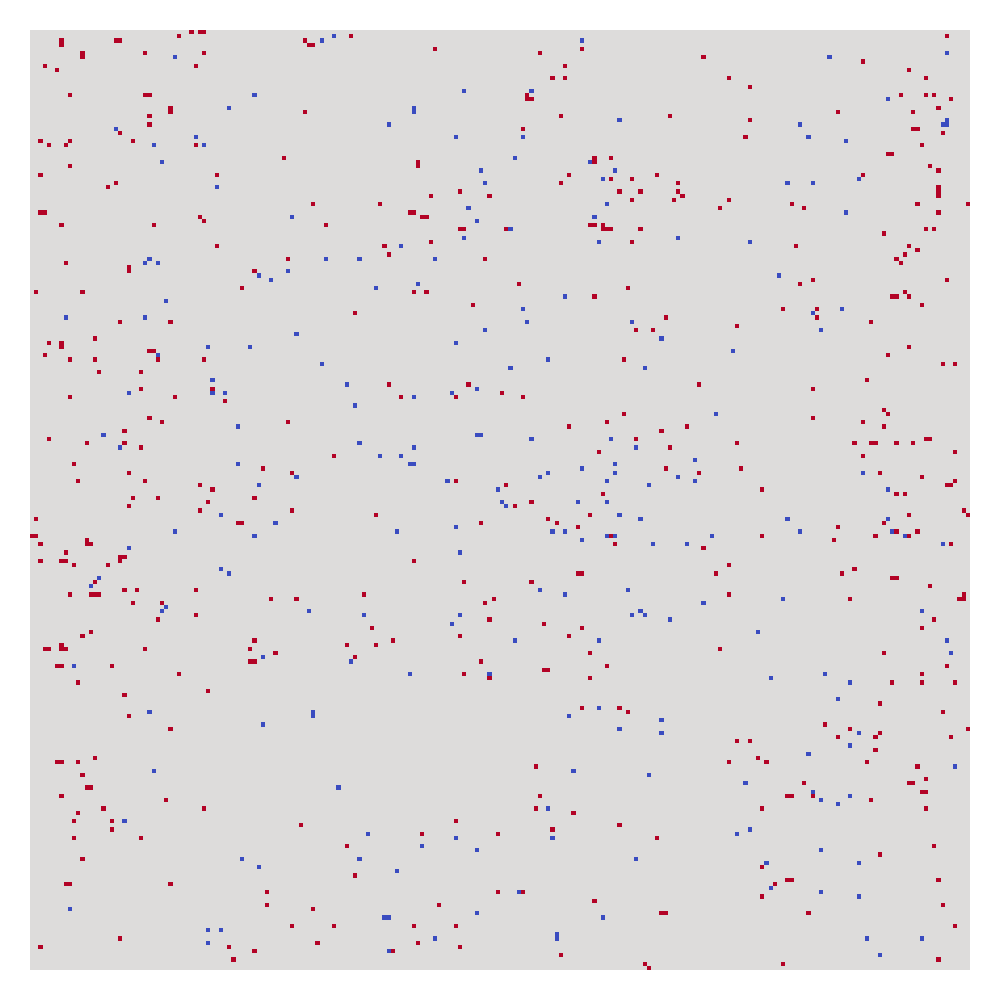
\includegraphics[height=1\linewidth]{01-images/05-resultate/uap_resnet18/uap0-resnet18-mri_data-n200-robustificationslevel1.png}
    \end{subfigure}\hfill%
    \begin{subfigure}{0.095\linewidth}
        \centering
        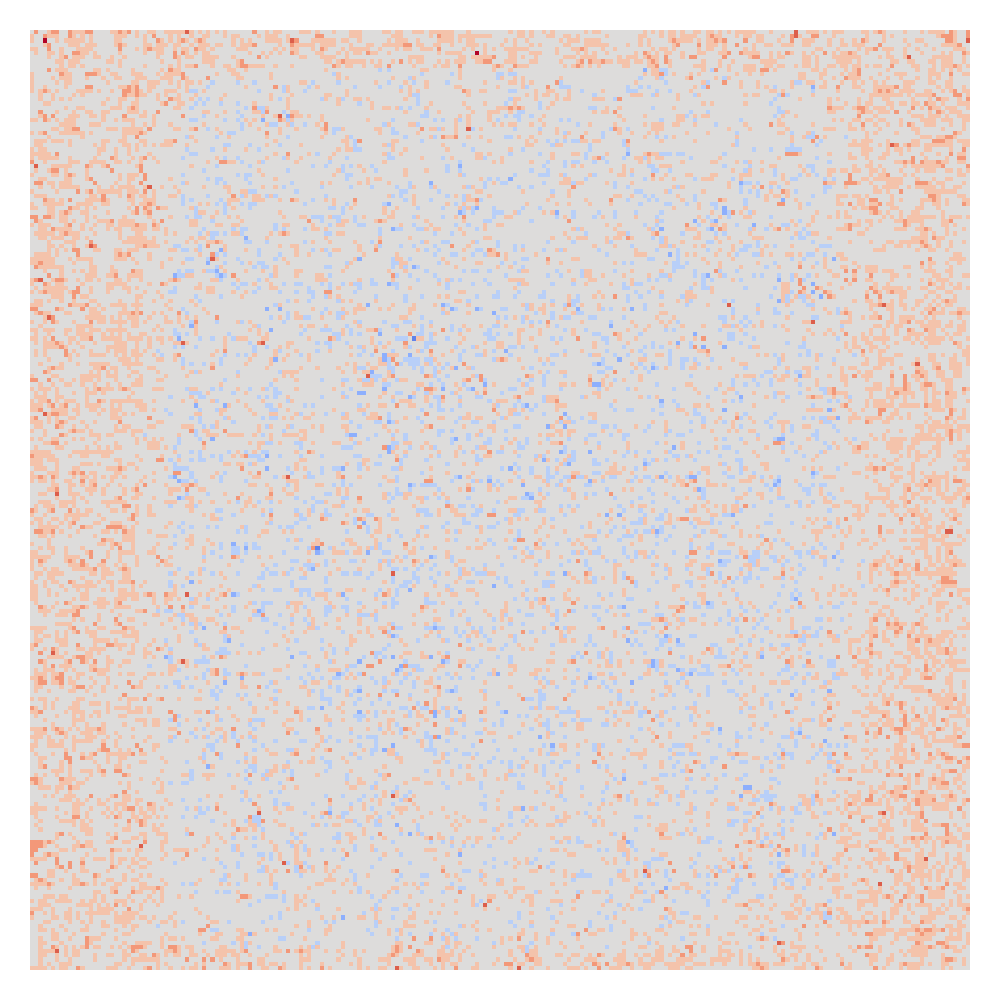
\includegraphics[height=1\linewidth]{01-images/05-resultate/uap_resnet18/uap0-resnet18-mri_data-n200-robustificationslevel2.png}
    \end{subfigure}\hfill%
    \begin{subfigure}{0.095\linewidth}
        \centering
        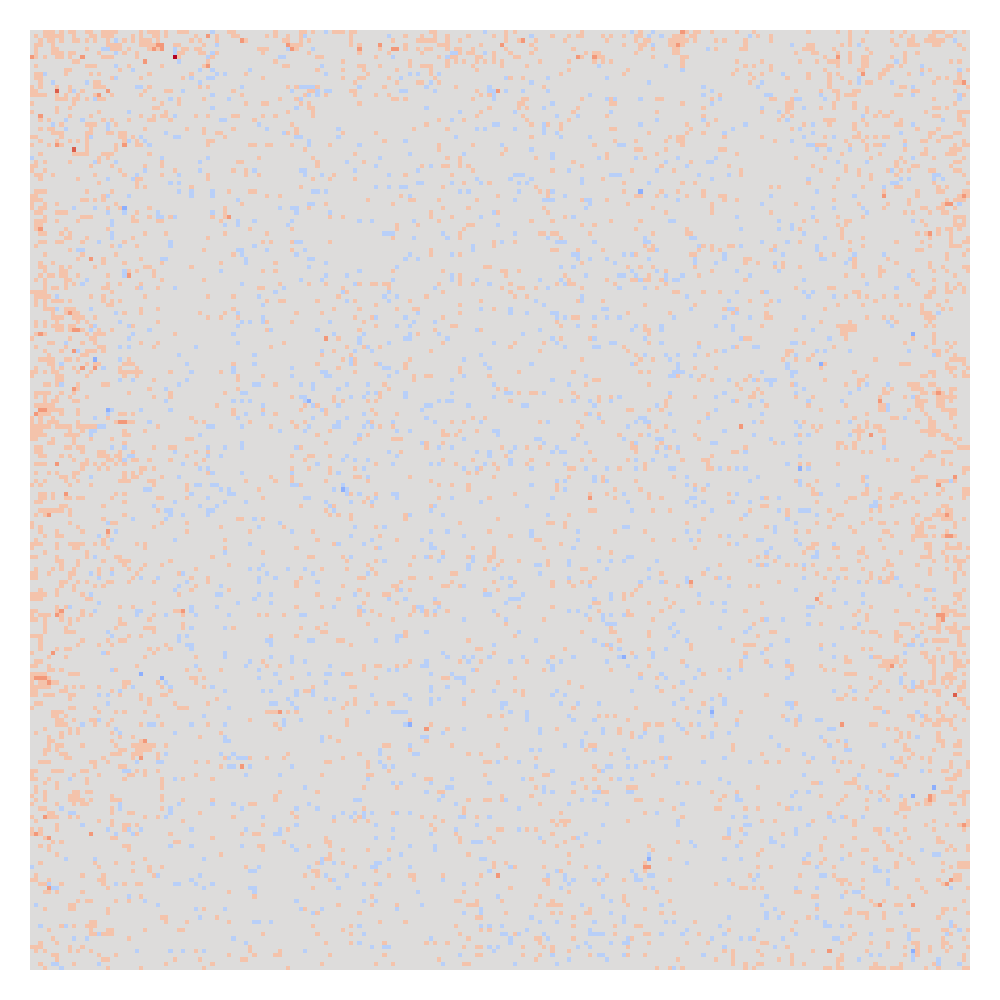
\includegraphics[height=1\linewidth]{01-images/05-resultate/uap_resnet18/uap0-resnet18-mri_data-n200-robustificationslevel3.png}
    \end{subfigure}\hfill%
    \begin{subfigure}{0.095\linewidth}
        \centering
        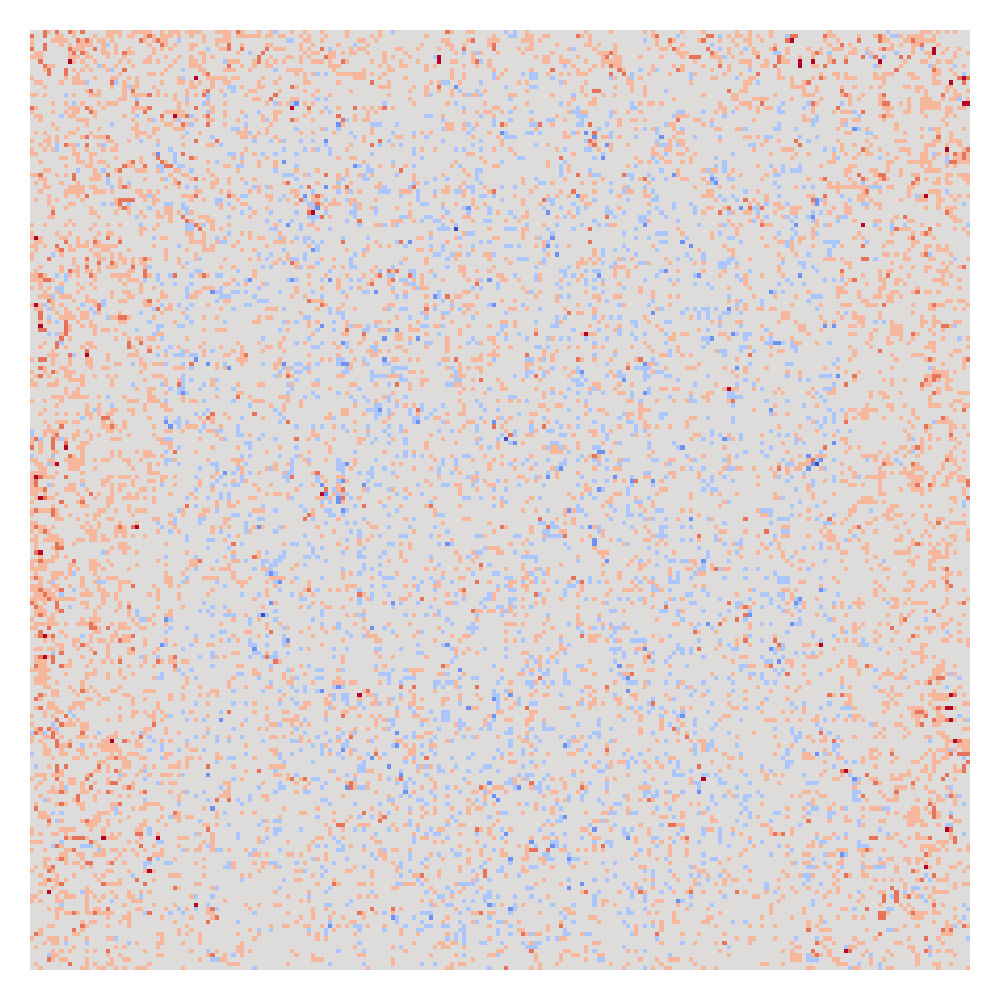
\includegraphics[height=1\linewidth]{01-images/05-resultate/uap_resnet18/uap0-resnet18-mri_data-n200-robustificationslevel4.png}
    \end{subfigure}\hfill%
    \begin{subfigure}{0.095\linewidth}
        \centering
        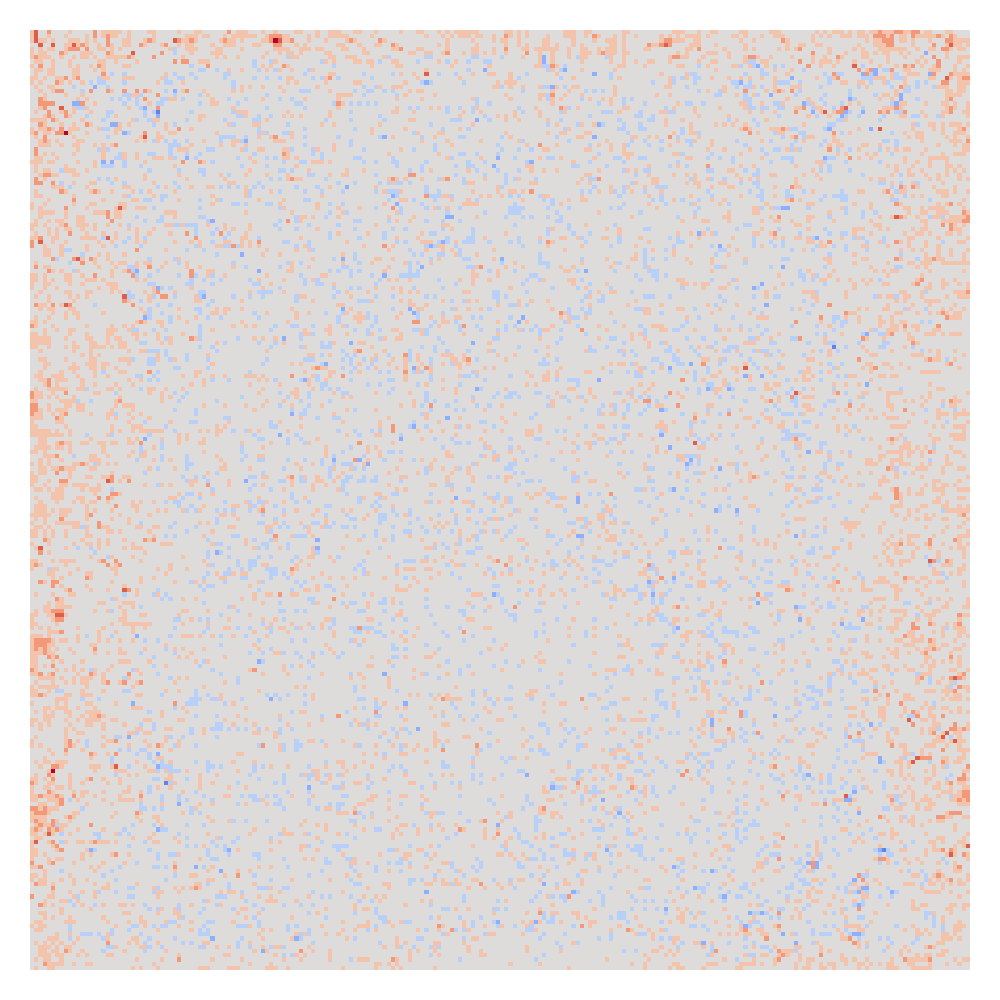
\includegraphics[height=1\linewidth]{01-images/05-resultate/uap_resnet18/uap0-resnet18-mri_data-n200-robustificationslevel5.png}
    \end{subfigure}\hfill%
    \begin{subfigure}{0.095\linewidth}
        \centering
        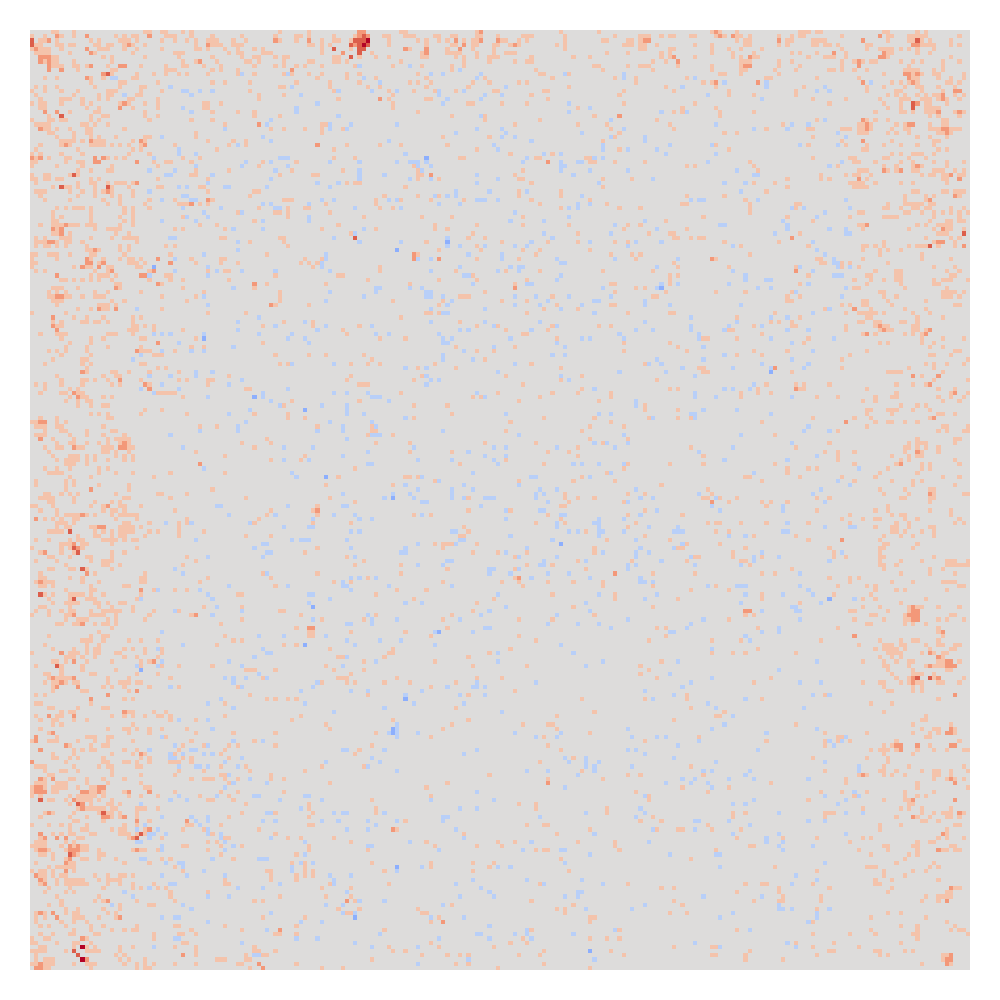
\includegraphics[height=1\linewidth]{01-images/05-resultate/uap_resnet18/uap0-resnet18-mri_data-n200-robustificationslevel6.png}
    \end{subfigure}
    \caption{Generierte UAPs des mit ResNet18 trainierten Hirntumor Datensatzes nach jedem Robustifikationslevel durch Adversarial Training von links nach rechts.}
    \label{fig:uap-verlauf-resnet18-mri-robustifikation}
\end{figure}




\subsubsection{UAP aus dem Paper}
Die UAP aus dem Paper wurden aus dem ImageNet Datensatz generiert. 
\begin{figure}[ht!]
    \centering
    \text{UAP vom Referenzpaper, Universal adversarial perturbations \cite{moosavi-dezfooli_universal_2017}} \\
    \begin{subfigure}{0.16\linewidth}
        \centering
        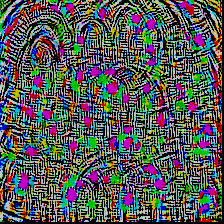
\includegraphics[height=1\linewidth]{01-images/05-resultate/uap_paper/uap-paper-caffeenet.png}
        \caption{CaffeeNet}
    \end{subfigure}\hfill%
    \begin{subfigure}{0.16\linewidth}
        \centering
        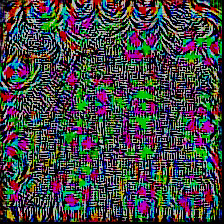
\includegraphics[height=1\linewidth]{01-images/05-resultate/uap_paper/uap-paper-vgg-F.png}
        \caption{VGG-F}
    \end{subfigure}\hfill%
    \begin{subfigure}{0.16\linewidth}
        \centering
        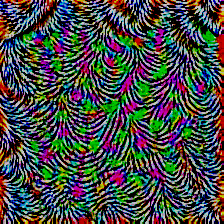
\includegraphics[height=1\linewidth]{01-images/05-resultate/uap_paper/uap-paper-vgg16.png}
        \caption{VGG-16}
    \end{subfigure}\hfill%
    \begin{subfigure}{0.16\linewidth}
        \centering
        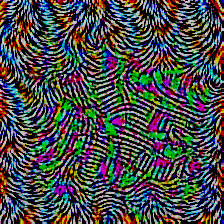
\includegraphics[height=1\linewidth]{01-images/05-resultate/uap_paper/uap-paper-vgg19.png}
        \caption{VGG-19}
    \end{subfigure}\hfill%
    \begin{subfigure}{0.16\linewidth}
        \centering
        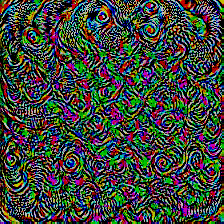
\includegraphics[height=1\linewidth]{01-images/05-resultate/uap_paper/uap-paper-googlenet.png}
        \caption{GoogLeNet}
    \end{subfigure}\hfill%
    \begin{subfigure}{0.16\linewidth}
        \centering
        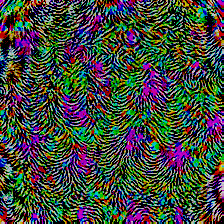
\includegraphics[height=1\linewidth]{01-images/05-resultate/uap_paper/uap-paper-resnet152.png}
        \caption{Res-Net152}
    \end{subfigure}
    \caption{Beispiele von UAP aus dem Paper Universal Adversarial Attacks \cite{moosavi-dezfooli_universal_2017}}
    \label{fig:referenzuap}
\end{figure}